% LLNCS macro package for Springer Computer Science proceedings;
% Version 2.21 of 2022/01/12
%
\documentclass[runningheads]{llncs}
%
\usepackage[T1]{fontenc}
% T1 fonts will be used to generate the final print and online PDFs,
% so please use T1 fonts in your manuscript whenever possible.
% Other font encondings may result in incorrect characters.
%v
\PassOptionsToPackage{table,xcdraw}{xcolor}
\usepackage{xcolor}
\usepackage{graphicx}
\usepackage{booktabs}
\usepackage{tikz}
\usepackage{fontawesome5}
\usetikzlibrary{trees, positioning, fit, shapes, arrows.meta, matrix,calc,shapes.geometric,shapes.misc}
\usepackage[nolist]{acronym}
\usepackage[hidelinks]{hyperref}
\usepackage{bookmark}
\usepackage{svg}
\usepackage{array}
\usepackage{amsmath}
\usepackage{amssymb, mathtools}
\usepackage{diagbox}
\usepackage{listings}
\usepackage{subcaption}  % Needed for subfigure support
\usepackage{float}
\usepackage{enumitem}

\newcommand{\todo}[1]{{\bf\color{red} Todo: #1}}
\newcommand{\klara}[1]{{\bf\color{blue!50!black} Klara: #1}}
\newcommand{\domi}[1]{{\bf\color{purple!80!black} Domi: #1}}
\renewcommand{\sectionautorefname}{Section}
\renewcommand{\subsectionautorefname}{Subsection}

\let\subset\subseteq
\let\supset\supseteq

\usepackage{csquotes}
\MakeOuterQuote{"}

% for code listings
\definecolor{codegreen}{rgb}{0,0.6,0}
\definecolor{codegray}{rgb}{0.5,0.5,0.5}
\definecolor{codepurple}{rgb}{0.58,0,0.82}
\definecolor{backcolour}{rgb}{0.95,0.95,0.92}

\lstdefinestyle{mystyle}{
    backgroundcolor=\color{backcolour},
    commentstyle=\color{codegreen},
    keywordstyle=\color{magenta},
    numberstyle=\tiny\color{codegray},
    stringstyle=\color{codepurple},
    basicstyle=\ttfamily\footnotesize,
    breakatwhitespace=false,
    breaklines=true,
    captionpos=b,
    keepspaces=true,
    numbers=left,
    numbersep=5pt,
    showspaces=false,
    showstringspaces=false,
    showtabs=false,
    tabsize=2
}

\lstset{style=mystyle}


%
\begin{document}
\newcommand{\authorA}{Klara M. Gutekunst}
\newcommand{\authorB}{Dominik Dürrschnabel}
\newcommand{\authorC}{Stefan Schneider}
\newcommand{\authorD}{Martin Potthast}

\newcommand{\emailA}{klara.gutekunst@uni-kassel.de}
\newcommand{\emailB}{dominik.duerrschnabel@mosbach.dhbw.de}
\newcommand{\emailC}{stefan.schneider@sschneider.de}
\newcommand{\emailD}{martin.potthast@uni-kassel.de}
%
\title{Hierarchical Background Knowledge in FCA via Must-Link-Before Constraints}
\titlerunning{Hierarchical Background Knowledge in FCA}
%
%\titlerunning{Abbreviated paper title}
% If the paper title is too long for the running head, you can set
% an abbreviated paper title here
%
\author{\authorA{}\inst{1,2}{\small \orcidID{0009-0002-6416-7873}}
        \and \authorB{}\inst{3}{\small \orcidID{0000-0002-0855-4185}}
        \and \authorC{}\inst{4}{\small \orcidID{0000-0001-6572-5983}}
        \and \authorD{}\inst{1,2}{\small \orcidID{0000-0003-2451-0665}}
}

%
\authorrunning{\authorA{}
        et al.
}
% copied from paper before, please update and add missing information
\institute{Deep Semantic Learning Group, University of Kassel, Germany
        % \and Knowledge \& Data Engineering Group, University of Kassel, Germany
        \and Interdisciplinary Research Center for Information System Design,
        \mbox{University of Kassel, Germany} \\%
        \and Baden-Wuerttemberg Cooperative State University Mosbach 
        \and Otto-von-Guericke-Universität Magdeburg \\%
        % \email{\emailA{}\\ \emailB{}\\ \emailC{}\\ \emailD{}}
}
\maketitle              % typeset the header of the contribution

\begin{abstract}
% \ac{fca} enables the generation of concept hierarchies without requiring an expert ontology.
% This raises the question of whether the resulting hierarchy aligns with existing sources of knowledge. 
% To guide the construction of coherent concept hierarchies, prior work in constrained clustering introduces the use of hierarchical \ac{mlb} constraints.

    % 1. build a world: FCA and constrained clustering
    % 2. stress the problem: how do different knowledge sources align?
\ac{fca} enables the construction of concept hierarchies from formal contexts without requiring expert ontologies. 
Hierarchical expert knowledge can be encoded through \ac{mlb} constraints in constrained clustering.
However, it remains unclear how agreement between hierarchies derived from heterogeneous knowledge sources can be quantified systematically.

% first contribution
In this work, we prove that \acs{mlb} constraints induce a valid closure operator, providing a theoretical foundation for incorporating hierarchical expert knowledge into \ac{fca}. 
% second contribution
Building on this result, we introduce a method for comparing concept lattices derived from \acs{mlb} constraints and data-driven topic models. 
% case study
Using the BankSearch dataset, we compare concept lattices derived from expert-defined \acs{mlb} constraints and a \acl{lda}-based document-topic context. We analyze their agreement through \textit{consistency} and \textit{coherence} lattice intersections at different levels of coherence.
Our analysis reveals distinct structural differences between both hierarchies, highlighting the need for relaxed coherence measures when integrating heterogeneous knowledge sources.

% redundant
% In this work, we introduce a method for comparing and integrating knowledge derived from \acs{mlb} constraints with an additional hierarchical knowledge source. 
% To evaluate the benefits of our approach, we conduct experiments on the BankSearch dataset and explore the universe of a closure operator provided by the \acs{mlb} constraints.
% These constraints are derived from a manually annotated topic hierarchy and subsequently mapped onto the corresponding document corpus.
% As our supplementary hierarchical knowledge source, we employ a \acl{lda} topic model, which constructs a document-topic context through statistical inference over the same corpus.

% We mathematically prove that MLB constraints induce a valid closure operator, providing the theoretical foundation for integrating hierarchical expert knowledge into FCA. 
% We then analyze the structural differences between the concept lattices guided by the two knowledge sources. 
% The influence of both knowledge bases is assessed qualitatively through manual review and quantitatively by analyzing their intersection for different levels of required coherence.
% We find distinct structural variations between the two concept lattices, reflected in their \textit{consistency} and \textit{coherence} lattice intersection.
% Our findings suggest a significant divergence between expert-defined hierarchies and data-driven topics, highlighting the necessity of relaxed coherence measures for practical knowledge integration.

\keywords{\acl{fca} \and Constraints \and Topic Modeling.}
\end{abstract}

\section{Introduction}
\label{sec:introduction}

% WORDNET: manual creation cf. le2019inferring, hearst1992hyponyms; hyponym = is-a relationship cf. hearst1992hyponyms
Concept hierarchies form the backbone of many expert ontologies.
In linguistic and lexical-semantic ontologies, they organize hyponym relationships under a common top node~\cite{le2019inferring} and structure information into categories, thereby supporting rule formulation as well as the retrieval from and reuse of knowledge bases~\cite{cimiano_learning_2005,yang2012personalized}.
However, the manual construction of high-quality domain-specific ontologies is costly and typically reflects only a snapshot of evolving knowledge~\cite{li2018unsupervised}.
Although manually curated ontologies are often regarded as the gold standard, automatic generation is desirable to reduce time and cost~\cite{Aznag2014LeveragingFC,risch2020hierarchical}.

% semantic dictionaries (Roget's Thesaurus)
% lexical databases (WordNet, FrameNet)
% Proof of concept on German prefices sporleder2002galois
% Proof of concept on inflectional properties of German nouns petersen:04
% reports on domestic violence (report id=obj, phrase=attr) Elzinga:09
% 1. intro to automatic concept hierarchy generation
Automatic concept hierarchy generation provides a scalable alternative and enables coverage of domains not represented in existing ontologies.
% 2. already structured data sources
Structured linguistic resources, such as the semantic dictionary Roget's Thesaurus~\cite{Priss:2004,old:04,Priss:96}, lexical databases such as WordNet~\cite{Priss:96,priss:98,GalnPez2014DiscoveringNS} and FrameNet~\cite{val:05}, and morphological feature systems~\cite{sporleder:02,petersen:04}, can be represented as formal contexts.
% 3. unstructured data sources, e.g., hearst1992hyponyms with Hearst patterns: automatically extract hyponym–hypernym relations; cimiano_learning_2005 with a multi-step NLP pipeline: parser/POS, lemmatizer ...
When applied to unstructured data sources such as text corpora, formal contexts must first be constructed from textual information. 
Approaches range from pattern-based extraction methods~\cite{hearst1992hyponyms,le2019inferring} to multi-step \acl{nlp} pipelines that derive binary object--attribute contexts from texts~\cite{cimiano_learning_2005}, as well as approaches using phrases directly as attributes~\cite{Elzinga:09}.
 


\ac{fca}-based concept hierarchy generation can be viewed as a form of conceptual clustering~\cite{Cimiano2004ComparingCD} that yields intensional descriptions of abstract concepts through their intents~\cite{cimiano_learning_2005}. 
Since each concept is characterized by an explicit set of shared attributes, the resulting hierarchy provides transparent, attribute-based explanations of the relationships between concepts, making \ac{fca}-based hierarchies inherently interpretable compared to similarity-based clustering methods.

Despite their scalability, automatically generated hierarchies may conflict with established expert ontologies, potentially reducing trust in either source.
Ensuring consistency with hierarchical background knowledge therefore requires mechanisms that guide and constrain the generation process.
Existing approaches (Section~\ref{sec:related_work}) include human-in-the-loop strategies~\cite{yang2012personalized}, the use of \aclp{llm}~\cite{kommineni2024from,zhang2025teleclass}, constrained \ac{fca}~\cite{belohlavek2011selecting,belohlavek2009formal,belohlavek2006formal,hidayat_constrained_fca_2024,mao_constrained_fca_2017}, and hierarchical constraints in similarity-based settings~\cite{bade2006personalized,bade_hierarchical_2014}. 

% Besides presentation purposes, \ac{fca} has been employed to identify potentially missing thesaurus entries in a specific expert ontology~\cite{zheng2020lexical,hao2021leveraging}. 

To date, the systematic integration of hierarchical background knowledge into \ac{fca}-based concept hierarchy generation through \ac{mlb} constraints has received limited attention.
We address this gap by incorporating \ac{mlb} constraints into the \ac{fca} framework to guide the construction of concept hierarchies (Section~\ref{sec:method}),\footnote{The code is available at \url{github.com/KlaraGtknst/fca-constrained-clustering}} thereby extending prior work that incorporates pairwise constraints~\cite{belohlavek2011selecting}.
In addition, we present a case study (Section~\ref{sec:case_study}) in which a concept lattice generated under \ac{mlb} constraints is compared to a concept lattice derived from an independent knowledge source using corpus-specific statistical topic modeling. 
The comparison is conducted across different levels of coherence, giving rise to the \textit{consistency} and \textit{coherence} lattices.

%\textcolor{red}{NOTE: Their conclusion includes future work on using humans for ontological relation validation (Attr. Explor.???). They also compare generated ontologies with human-modeled ontologies via Precision, Recall, F-measure...}

% Usually you
%Since this approach relies solely on syntactic structure present in the text corpus, the available knowledge is very limited.
%Hierarchical constraints can be thought of a tool to model certain degrees of certitude with respect to the information's validity.

\section{Related Work}
\label{sec:related_work}

% \subsubsection{Data-Driven Approaches}
% 1. Data-driven concept hierarchy generation from text corpora
% TODO: unclear opening
Automatic concept hierarchy generation from text corpora has been approached in various ways.
%% 1.1. Non-FCA data-driven approaches
Hierarchical text classification assigns documents one or more labels organized in a taxonomy~\cite{yu2022constrained}, implicitly creating a hierarchical structure of documents.
Approaches range from regularization-based classifiers~\cite{gopal2013recursive}, embedding-based document-label matching~\cite{li2019hiercon} to neural sequence models~\cite{risch2020hierarchical,yu2022constrained} and \ac{llm}-assisted taxonomy enrichment~\cite{zhang2025teleclass}.

%% 1.2. FCA-based data-driven approaches
Beyond classification-based approaches, research has explored deriving concept hierarchies directly from textual data using \ac{fca}.
Since \ac{fca}-based hierarchy generation can be viewed as conceptual clustering that yields intensional descriptions of abstract concepts via their intents~\cite{cimiano_learning_2005}, text corpora can be represented as a formal contexts in which documents form the objects and extracted features serve as attributes.
Feature sources include semantic dictionaries~\cite{Priss:2004,old:04,Priss:96}, lexical databases~\cite{Priss:96,priss:98,GalnPez2014DiscoveringNS,val:05}, morphological structures~\cite{sporleder:02,petersen:04}, bag-of-words representations capturing the presence of phrases~\cite{Elzinga:09,cigarran_twitter_fca_2016}, and latent topics derived from topic models~\cite{Aznag2014LeveragingFC,wang_topic_feature_2021,wang_topic_hierarchy_2023,hirth_ordinal_2024,gutekunst2025conceptual}.
% \acl{lda} topic features~\cite{wang_topic_feature_2021,wang_topic_hierarchy_2023}, and other topic model features~\cite{Aznag2014LeveragingFC,gutekunst2025conceptual,hirth_ordinal_2024}. % hirth_ordinal_2024 uses own trained topic model refered to as SSH21, but is something trained using non-negative matrix factorization, gutekunst2025conceptual use top2vec, Aznag2014LeveragingFC: compared LDA, CTM, PLSA (found LDA to be best)


% \subsubsection{Knowledge-Driven Approaches}
% 2. Knowledge-based concept hierarchy generation
% 2.1. Constrained Hierarchical Clustering -> explain MLB constraints
%% clustering with constraints
In constrained clustering, prior knowledge is expressed through constraints rather than derived from data.
% , which require objects to be in the same or different clusters, respectively.
Conventional constrained clustering methods typically operate on a single level of granularity~\cite{wagstaff2001constrained}.
%% limits of pairwise constraints: hierarchical clustering
However, pairwise \textit{must-link} and \textit{cannot-link} constraints become ambiguous in hierarchical clustering settings, where objects may belong to the same cluster at one hierarchy level but not at another~\cite{bade_hierarchical_2014}.
To address this limitation, Bade et al.~\cite{bade2006personalized,bade_creating_2008} introduce \ac{mlb} constraints for \ac{hac}.
These constraints encode relative hierarchical relationships through the order in which objects should be merged during agglomeration~\cite{bade2006personalized,bade_creating_2008,bade_hierarchical_2014}.
Existing approaches incorporate \ac{mlb} constraints by modifying similarity measures during merging~\cite{bade2006personalized}, delaying merges until constraint violations are resolved~\cite{zhao2010hierarchical}, or integrating them into matrix-based approaches~\cite{zheng2011semi}.

% In hierarchical clustering, two main approaches exist: partitional and agglomerative hierarchical clustering.
% While partitional hierarchical clustering build a hierarchy by recursively partitioning the data (i.e., top to bottom), agglomerative hierarchical clustering methods build a hierarchy by iteratively merging clusters (i.e., bottom to top)~\cite{zhao2002evaluation}.

% The \ac{hac} algorithm iteratively merges the two most similar clusters into one. The \ac{ihac} extends the \ac{hac} algorithm by not only considering similarity but also constraint violations~\cite{bade_hierarchical_2014}.

% MacLellan et al.~\cite{maclellan2024trestle} incrementally builds concept hierarchies.

% 2.2. Constrained and Knowledge-Guided FCA
Several works also investigate incorporating constraints or expert knowledge directly into \ac{fca}.
% constrained FCA != we use MLB constraints
Constraints have been used to encode mutually exclusive attributes~\cite{hidayat_constrained_fca_2024}
% we use support, i.e., the number of objects sharing a set of attributes, while belohlavek2009formal define importance directly on attributes, or belohlavek2006formal constrain closure operators, or mao_constrained_fca_2017 define a operator S (!= closure operator) to determine interesting attribute sets
and to prune concept lattices by retaining only concepts whose intents satisfy relevance criteria. These criteria have been defined through attribute properties~\cite{belohlavek2011selecting,belohlavek2009formal,hidayat_constrained_fca_2024}, constraints on the closure operator~\cite{belohlavek2006formal}, or additional operators~\cite{mao_constrained_fca_2017}. 
% Attribute Exploration with contradicting experts: != we do not only have shared implications but also some-what shared (i.e., coherence lattice)
Research has also extended Attribute Exploration to settings with multiple, potentially contradictory or incomplete experts, aiming to derive implications shared across different subsets of experts~\cite{felde2021triadic,felde2022attribute}.

%% Our work
However, prior work has incorporated hierarchical \ac{mlb} constraints mainly into traditional clustering methods rather than hierarchy construction via \ac{fca}. 
To the best of our knowledge, no comparison exists between concept lattices derived from probabilistic topic models and those derived from constraints.

\section{Foundations}
\label{sec:foundations}

% This section introduces the theoretical foundations underlying our approach. 
In Section~\ref{sec:foundations_fca}, we present the background on \ac{fca}, 
%which provides the formal framework for representing hierarchical structures.
and subsequently, in Section~\ref{sec:foundations_mlb}, we discuss \ac{mlb} constraints in constrained \ac{hac}. 

\subsection{\ac{fca}}
\label{sec:foundations_fca}

% \subsubsection{\ac{fca}} 
The mathematical theory of \ac{fca}~\cite{fca-book} is a method to analyze relational data in a hierarchical structure.
The triple $\mathbb{K} \coloneq (G, M, I)$ defines the \emph{formal context}.
$G$ is the set of \emph{objects}, $M$ is the set of \emph{attributes},
and $I \subseteq G \times M$ is the \emph{incidence relation}, which describes when an object $g$ has an attribute $m$.
The object derivation $(\cdot)' : \mathcal{P}(G) \to \mathcal{P}(M)$
defines for any subset $A \subseteq G $ as $A' \coloneq \{m \in M \mid \forall g \in A : (g, m) \in I\}$.
The attribute derivation $(\cdot)' : \mathcal{P}(M) \to \mathcal{P}(G)$ is
defined for any subset $B \subseteq M $ as $B' \coloneq \{g \in G \mid \forall m \in B : (g, m) \in I\}$.
The same notation $(\cdot)'$ is used for both derivation operators.
A formal concept of $\mathbb{K}$ is a pair $(A, B)$ where $A \subseteq G$ and $B \subseteq M$
satisfy the conditions $A' = B$ and $B' = A$.
% Hence, all objects in $A$ share the attributes described by $ B $.
The set $\mathfrak{B}(\mathbb{K})$ denotes all formal concepts of $\mathbb{K}$.
The concept lattice $\underline{\mathfrak{B}}(\mathbb{K}) \coloneq (\mathfrak{B}(\mathbb{K}), \leq)$ is defined by the set of all formal concepts with the order relation
$(A, B) \leq (C, D)$ if and only if $A \subseteq C$.
% forms an ordered set.
% More precisely, $\underline{B}(\mathbb{K})$ is a lattice.
% Hence, for any subset $C \subseteq \mathfrak{B}(\mathbb{K})$, both the greatest lower bound (meet) and the least upper bound (join) exist.
% Consequently, $\underline{\mathfrak{B}}(\mathbb{K})$ is referred to as the concept lattice.

% This lattice structure  enables a hierarchical organization of documents, terms, and topics in topic modeling,
% providing a formal foundation for understanding relationships between concepts in text analysis \cite{topic_modeling_2024}.


% \subsubsection{Canonical Basis}
(also: Duquenne-Guigues basis or stem basis \cite{ganter_conceptual_2016}).
A formal context $(G, M, I)$ can also be defined via a set of implications $\mathcal{L}$ that is sound (i.e., each implication in $\mathcal{L}$ holds in $(G, M, I)$), complete (i.e., each implication that holds in $(G, M, I)$ follows from $\mathcal{L}$), and nonredundant (i.e., no implication in $\mathcal{L}$ follows from other implications in $\mathcal{L}$).
The canonical basis is $\{P \rightarrow P'' \smallsetminus P | P$ is pseudo-closed$\}$.
A finite subset $P \subseteq M$ is pseudo-closed if and only if (i) $P \neq P''$ (i.e., $P$ is not closed and in other words: $P$ is not a concept intent) and (ii) if $Q \subsetneq P$ is a pseudo-closed proper subset of $P$, then $Q'' \subset P$ (i.e., $P$ contains the closure of every pseudo-closed subset with fewer elements).
If (i) and (ii) holds true, $P$ is a pseudo-intent of $(G, M, I)$.
The canonical basis is nonredundant, i.e., no implication in the canonical basis is dispensable.
It is not the only implication basis, but there is no implication basis with fewer implications \cite{ganter_conceptual_2016}.

\newcommand{\latticeToMLB}{%
\begin{figure}[t]
\centering
\resizebox{0.85\textwidth}{!}{%
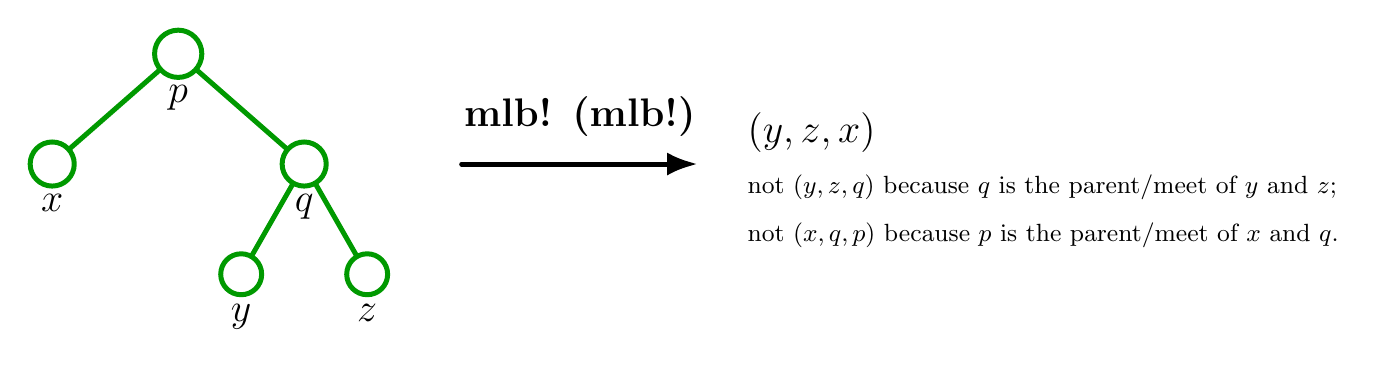
\begin{tikzpicture}[
  >=Latex,
  line cap=round, line join=round,
  thick,
]
  % --- styles
  \colorlet{nodegreen}{green!60!black}
  \tikzset{
    gedge/.style={draw=nodegreen, line width=1.8pt},
    gnode/.style={draw=nodegreen, fill=white, line width=1.8pt},
    arrow/.style={->, line width=1.8pt, draw=black},
    lbl/.style={font=\Large},
  }

  % --- coordinates (tree on the left)
  \coordinate (n1) at (0,2.8);
  \coordinate (n2) at (-1.6,1.4);
  \coordinate (n3) at ( 1.6,1.4);
  \coordinate (n4) at ( 0.8,0.0);
  \coordinate (n5) at ( 2.4,0.0);

  % --- green edges
  \draw[gedge] (n1) -- (n2);
  \draw[gedge] (n1) -- (n3);
  \draw[gedge] (n3) -- (n4);
  \draw[gedge] (n3) -- (n5);

  % --- green open nodes
  \draw[gnode] (n1) circle [radius=0.30];
  \draw[gnode] (n2) circle [radius=0.28];
  \draw[gnode] (n3) circle [radius=0.28];
  \draw[gnode] (n4) circle [radius=0.26];
  \draw[gnode] (n5) circle [radius=0.26];

  % --- labels (node numbers)
  \node[lbl, anchor=south] at ($(n1)+(0,-0.85)$) {$p$};
  \node[lbl, anchor=north] at ($(n2)+(0,-0.25)$) {$x$};
  \node[lbl, anchor=north] at ($(n3)+(0,-0.25)$) {$q$};
  \node[lbl, anchor=north] at ($(n4)+(0,-0.25)$) {$y$};
  \node[lbl, anchor=north] at ($(n5)+(0,-0.25)$) {$z$};

  % --- middle arrow + label
  \coordinate (Astart) at (3.6,1.4);
  \coordinate (Aend)   at (6.6,1.4);
  \draw[arrow] (Astart) -- (Aend);
  \node[font=\bfseries\Large] at ($(Astart)!0.5!(Aend)+(0,0.6)$) {\ac{mlb}};

  % --- right-side explanation (siblings + uncle)
  \node[anchor=west, font=\Large] at (7.1,1.8) {$(y,z,x)$};
  \node[anchor=west, font=\Large] at (7.1,1.1)
    {\small not $(y,z,q)$ because $q$ is the parent/meet of $y$ and $z$;};
  \node[anchor=west, font=\Large] at (7.1,0.5)
    {\small not $(x,q,p)$ because $p$ is the parent/meet of $x$ and $q$.};

\end{tikzpicture}%
}
\caption{Building \ac{mlb} constraints using the ``siblings + uncle'' rule, where siblings $y,z$ are connected to the same parent node $q$ and $x$ is the uncle node.}
\label{fig:concept_lattice2mlb}
\end{figure}%
}

\subsection{\acl{mlb} Constraints}
\label{sec:foundations_mlb}

Clustering structures unlabelled data, which is particularly useful in real-world applications where labeled data is scarce and annotation is costly. 
Clustering algorithms group data points according to a similarity criterion, typically minimizing intra-cluster distances while maximizing inter-cluster distances.
Prior knowledge about the dataset can be incorporated through constraints. 
The simplest forms are pairwise \textit{must-link} and \textit{cannot-link} constraints, enforcing that two instances must or must not belong to the same cluster. 
However, pairwise constraints generally apply only at one level of granularity.

Hierarchical clustering instead organizes data into nested groups at different levels of granularity~\cite{bade_hierarchical_2014}. 
To incorporate prior knowledge in this setting, \ac{mlb} constraints specify the relative agglomeration order of three data points $d_x$, $d_y$, $d_z$. 
An \ac{mlb} constraint
\begin{eqnarray}
    MLB_{x y z} = (d_x, d_y, d_z)
    \label{eq:mlb_xyz}
\end{eqnarray}
states that $d_x$ and $d_y$ should be merged before either is merged with $d_z$, where $d_x$ and $d_y$ are symmetric. 
Let $H = (C, \prec, \text{root})$ denote a cluster hierarchy, where $C$ is a set of clusters, $\prec$ is a strict partial order over $C$ representing the parent-child relation, and $\text{root} \in C$ is the root cluster~\cite{bade_hierarchical_2014}. 
Definitions~\eqref{def:mlb_implication} and \eqref{def:mlb_counterexample} formalize the idea that $d_x$ and $d_y$ are more closely related in the hierarchy than $d_x$ and $d_z$. 
\autoref{fig:hierarchy_to_mlb} illustrates valid \ac{mlb} constraints for a toy example.

\begin{definition}[\ac{mlb} Implication]
    \label{def:mlb_implication}\\
    Given \ac{mlb} constraint $MLB_{x y z}$:
    $\forall c \in H: d_x \in c \wedge d_z \in c \rightarrow d_y \in c$
\end{definition}
\begin{definition}[\ac{mlb} Counter Example]
    \label{def:mlb_counterexample}\\
    Given \ac{mlb} constraint $MLB_{x y z}$:
    $\exists c \in H: d_x \in c \wedge d_y \in c \wedge d_z \notin c$
\end{definition}

\hierarchyToMLB{}

% A \ac{mlb} constraint for hierarchical clustering can be transformed into multiple pairwise constraints for partitional clustering by adding one must-link constraint between $d_x$ and $d_y$ and two cannot-links between $d_x, d_z$ and $d_y, d_z$~\cite{bade_hierarchical_2014}.

% \subsubsection{Concept hierarchies} 
% Concept hierarchies structure information into hierarchies and facilitate working with knowledge-bases~\cite{cimiano_learning_2005}.


% \subsubsection{Attribute Exploration}
\label{subsec:basic_ae}
Attribute exploration tries to build the implication theory (i.e., set of implications true for all objects) of the entire domain.
Every implication that holds true for all objects follows from the canonical basis.
For every implication that does not hold in general, there is a counterexample among the objects.
The exploration algorithm repeatedly asks the domain expert about undecided formulas either confirming them or disproving them by extending the object set with additional evidence \cite{ganter_conceptual_2016}.

% \subsubsection{Incomplete knowledge}
\label{subsec:incomplete_knowledge}
An incomplete lattice is a ternary context $(G,M,W,I)$ with values $W=\{\times, ?, \circ\}$ where $? < \times$ and $? < \circ$.
$<$ is an order over the amount of information.
$I(g,m)=?$ symbolizes the lack of knowledge about the relation between object $g$ and attribute $m$ \cite{holzer_incompleteFCA_2001}.
\textcolor{red}{TODO: \cite{hille_incomplete_2025,burmeister_treatment_2000}}


\section{Method}
\label{sec:method}
% defines commands used below to insert datastructure (for better readability)
\newcommand{\formalcontexttable}{%
\begin{table}[]
\centering
\caption{Formal context}
\label{tab:formal_context}
\begin{tabular}{|l|c|c|c|c|c|}
\hline
          & $x_A$           & $x_B$           & $x_C$           & $x_D$           & \dots \\ \hline
$c_1$         & $\times$    & $\times$    &             &             &        \\ \hline
$c_2$         &             &             & $\times$    & $\times$    &        \\ \hline
$c_1 \vee c_2$ & $\times$    & $\times$    & $\times$    & $\times$    &        \\ \hline
$\vdots$      &             &             &             &             & $\ddots$ \\ \hline
\end{tabular}%
\end{table}%
}

\newcommand{\dendogram}{%
\begin{figure}[]
\centering
\caption{Dendrogram with objects on the bottom.}
\label{fig:dendrogram}

\begin{tikzpicture}[scale=1]
% Positions of objects (bottom)
\node (A) at (0,0) {$x_A$};
\node (B) at (2,0) {$x_B$};
\node (C) at (4,0) {$x_C$};
\node (D) at (6,0) {$x_D$};

% Merge A and B
\coordinate (ABtop) at (1,1);
\draw (A) -- (0,1) -- (ABtop) -- (2,1) -- (B);

% Merge C and D
\coordinate (CDtop) at (5,1);
\draw (C) -- (4,1) -- (CDtop) -- (6,1) -- (D);

% Merge AB and CD
\coordinate (root) at (3,2);
\draw (ABtop) --(1,2) -- (5,2) -- (CDtop);

\end{tikzpicture}
\end{figure}
}

\newcommand{\lattice}{%
\begin{figure}[h]
\centering
\caption{Concept lattice for the transposed formal context.}
\label{fig:concept_lattice}

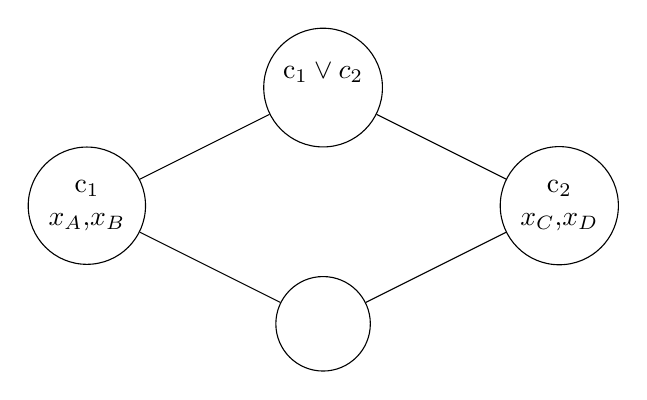
\begin{tikzpicture}[scale=1, every node/.style={draw, circle, align=center, minimum width=1.2cm, minimum height=1.2cm}]
% Nodes
\node (top) at (0,3) {c$_1 \vee c_2$ \\ };
\node (left) at (-3,1.5) {c$_1$ \\ $x_A$,$x_B$};
\node (right) at (3,1.5) {c$_2$ \\ $x_C$,$x_D$};
\node (bottom) at (0,0) {};

% Edges
\draw (top) -- (left);
\draw (top) -- (right);
\draw (left) -- (bottom);
\draw (right) -- (bottom);

\end{tikzpicture}
\end{figure}
}


\subsection{\acs{mlb} constraints and \acs{fca}}

Implications are usually defined on attribute sets rather than on object sets \cite{fca-book}, but we will work with object exploration since it aligns directly with constrained hierarchical clustering.
\textcolor{gray}{The methodology proposed is directly applicable to both versions, differing only by the necessity of transposing the context for visualization via concept lattices.}
We denote the data points $\mathcal{D}=\{d_A, d_B, d_C, d_D, \dots\}$ the set of objects $G$ and the clusters $c_i \in \mathcal{C}$ the set of attributes $M$. 
For simplicity, we explain our idea on the toy example given in \autoref{tab:formal_context}.
\formalcontexttable{}

The corresponding hierarchical cluster is given as a dendrogram in \autoref{fig:dendrogram}.
The bottom elements are data points in $\mathcal{D}$.
Iterative merging of clusters are indicated by agglomerating lines from the bottom to the top.
\dendogram{}

There are two directions to consider for proving the equivalence of both presentations.
First, we will outline how a hierarchical cluster can be turned into its corresponding formal context and next, we will describe the other direction.
In the following, we will describe the hierarchical cluster as a dendrogram.

\subsubsection{Hierarchical cluster to formal context.}
For each cluster on the lowest hierarchical level, i.e., the lowest line between leaf elements, add an attribute $c_i$ with $i > |\mathcal{C}|$. 
Next, update the incidence relation $I = I \cup \{ d | d \in c_i\}$, i.e., add each data point $d$ of that cluster to the new attribute's extent, such that $(c_i)'$ contains all data points of that cluster. 
Once all lower clusters have been processed, proceed with the next higher cluster hierarchy.
For each cluster emerging from sub-clusters $c_i, c_j \in \mathcal{C}$, add a new attribute $c_i \vee c_j$.
This attribute's extent contains all attributes in either one of the sub-cluster's extents, i.e., $(c_i \vee c_j)' = (c_i)'\cup(c_j)'$.
Proceed likewise for all clusters on that hierarchy and repeat the process for higher level emerging clusters.


\subsubsection{Formal context to hierarchical cluster.}
Given a formal context $(G,M,I)$ where $G$ denotes the set of data points $\mathcal{D}$ and $M$ denotes the set of clusters $c_i \in \mathcal{C}$, all objects $d \in G$ are leaf nodes of the dendogram.
For each attribute $a_i \in M$, identify any other attributes $a_j \in M$ whose extent is a superset of $a_i$'s extent.
Save those attributes in a successor list (or better: set) $s_{a_i}$.
% one could omit transitive constraints, but not necessary
To keep track of already processed cluster attributes, initialize a list $processed$.
To keep track of the constraints add a list of resulting constraints $r$.
%
Next, select one attribute $a_i$ with minimal extent cardinality $|(a_i)'|$, i.e., the smallest cluster.
For any pair of objects in $a_i$'s extent, i.e. data points $d_i, d_j \in (a_i)'$, add a pairwise \texttt{must-link} constraint to $r$.
To capture the hierarchical relation between the clusters, for $d_i, d_j$ and any object $d_k$ in $a_i$'s successor list's items' extent excluding $d_i, d_j$, i.e., data point $d_k \in (a)'\smallsetminus \{d_i, d_j\}$ for attribute $a \in s_{a_i}$, add a \texttt{\ac{mlb}} constraint $MLB_{d_i, d_j, d_k}$.
Once all \ac{mlb} constraints for the pair $d_i, d_j$ and objects $d_k \in (a)'\smallsetminus \{d_i, d_j\}$ have been added, the next pair in $(a_i)'$ can be processed.
Once all pairs in $(a_i)'$ have been processed, $a_i$ is added to $processed$.
Repeat the steps for the next attribute $a_j$, i.e., cluster, with minimal extent cardinality $|(a_j)'|$ which has not yet been processed, i.e., is not element of $processed$ is selected.
The algorithm ends once all cluster attributes have been added to $processed$. 
%
The resulting set of \ac{mlb} constraints is models the solution space of possible clusters.
Any clustering algorithm, i.e., including \ac{hac} and \ac{ihac}, that respects these \textit{hard} constraints can produce a possible solution that lives within this solution space.

\subsubsection{Formal context to concept lattice.}
Given a formal context $(G,M,I)$ where $G$ denotes the set of data points $\mathcal{D}$ and $M$ denotes the set of clusters $c_i \in \mathcal{C}$, we can compute a meaningful concept lattice representation.
The resulting concept lattice for the formal context in \autoref{tab:formal_context} is given in \autoref{fig:concept_lattice}.

\lattice{}

\subsection{Deriving Formal Contexts from Datasets}
\textcolor{red}{TODO: How do we get the input (G, M, I) from which Datasets?
Each document is exactly mapped to one category / topics:
\cite{bade_hierarchical_2014}
\begin{itemize}
    \item BankSearch Dataset
    \item Reuters Dataset (old)
\end{itemize}
Each document is cannot been mapped exactly to one category (but multiple):
\begin{itemize}
    \item Reuters Dataset (new)
\end{itemize}
Expert Ontology as reference:
\begin{itemize}
    \item WordNet \cite{fellbaum2010wordnet}
\end{itemize}
Probably same considerations on research designs by using object attribute matrices consisting of documents and topics exists.
\cite{ceulemans_detecting_2010}
}

\subsection{Deriving \ac{mlb} constraints from categories}

\textcolor{red}{BankSearch:}
Hierarchies occur naturally in data, often in the form of structural organisation in a file system or by personal topic hierarchies~\cite{bade_creating_2008}.
\ac{mlb} constraints can be derived as illustrated in Figure~\ref{fig:derive_mlb_constraints}.

\deriveMLBconstraints{}

\subsection{External Knowledge}

Besides existing file structures, we employed external knowledge bases such as WordNet~\cite{fellbaum2010wordnet} and topic models~\cite{gutekunst2025conceptual} for enriching the dataset with categories.

\subsubsection{WordNet}
Synsets etc.~\cite{fellbaum2010wordnet}
WordNet can be used to derive constraints from expert ontologies by mapping each category term (lemma) to the synsets (senses) in which it appears and then exploiting ``IS-A'' relations between synsets: terms that share a synset can yield synonymy-based must-link constraints (cf. Figure~\ref{fig:wordnet-must-link-constraints}), and terms whose synsets are connected by an ``IS-A'' path can yield hierarchical constraints (cf. Figure~\ref{fig:wordnet-mlb-constraints}) whose strength depends on the shortest path distance to a common ancestor. 
\begin{figure}[t]
    \centering
    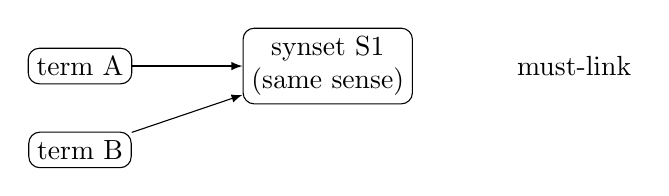
\begin{tikzpicture}[
        term/.style={draw, rounded corners, align=center, inner sep=3pt},
        rel/.style={->, >=latex}
    ]
        % Same synset -> must-link constraint
        \node[term] (a) {term A};
        \node[term, below=6mm of a] (b) {term B};
        \node[term, right=14mm of a] (s1) {synset S1\\(same sense)};
        \node[align=center, right=12mm of s1] {must-link};
        \draw[rel] (a) -- (s1);
        \draw[rel] (b) -- (s1);

    \end{tikzpicture}
    \caption{Deriving constraints from shared synsets in WordNet.}
    \label{fig:wordnet-must-link-constraints}
\end{figure}
\begin{figure}[t]
    \centering
    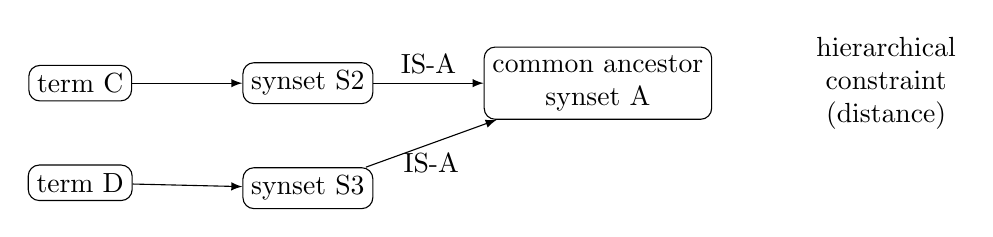
\begin{tikzpicture}[
        term/.style={draw, rounded corners, align=center, inner sep=3pt},
        rel/.style={->, >=latex}
    ]

        % Connected synsets -> hierarchical constraint
        \begin{scope}[xshift=80mm]
            \node[term] (c) {term C};
            \node[term, below=8mm of c] (d) {term D};
            \node[term, right=14mm of c] (s2) {synset S2};
            \node[term, below=8mm of s2] (s3) {synset S3};
            \node[term, right=14mm of s2] (anc) {common ancestor\\synset A};
            \node[align=center, right=12mm of anc] {hierarchical\\constraint\\(distance)};
            \draw[rel] (c) -- (s2);
            \draw[rel] (d) -- (s3);
            \draw[rel] (s2) -- node[above]{IS-A} (anc);
            \draw[rel] (s3) -- node[below]{IS-A} (anc);
        \end{scope}
    \end{tikzpicture}
    \caption{Deriving constraints from connected ``IS-A'' chains in WordNet.}
    \label{fig:wordnet-mlb-constraints}
\end{figure}
This mapping also provides a coverage signal, because terms absent from any synset cannot be constrained through WordNet. 
In our analysis, coverage is high, and if ``groups'' is empty, there are no overlapping synsets among category terms.
Although about 3000 shared ``IS-A'' chains exist, only 22 term pairs have distance 1, so the strongest hierarchical relations are sparse. 
These observations highlight limitations: constraints are only obtainable for terms represented in WordNet; must-link constraints may be unavailable if categories do not share synsets; and ``IS-A''/\ac{mlb} constraints can be weak when common ancestors are distant, which reduces their practical discriminative power and may introduce noise in constraint strength estimation.

\subsubsection{Topic Models}

A topic model is a generative model for documents, where documents are mixtures of $K$ topics and topics are mixtures of words (i.e., multinomial distribution over a word vocabulary).
Topic models rely on the bag-of-words assumption, i.e., ignoring the order of words.
We employed gensim's \ac{lda}\footnote{\url{https://radimrehurek.com/gensim/models/ldamodel.html} (30.12.2025)}.
\ac{lda} is unsupervised and based on statistical bayesian topic models~\cite{alghamdi_survey_2015}.

We build 200 latent topics across the data corpus, and extract the 10 most dominant topics per document each represented by the 10 most probable words per topic.
The resulting structure is \texttt{\{document $d_1$: [topic $t_{11}$: [word $w_{t_{11}-1}$, \dots, word $w_{t_{11}-10}$], topic $t_{12}$ \dots], document $d_2$:\dots \}}.
The number of initial topics (i.e., 200) is chosen arbitrarily.


% \input{chapters/07_implementation}

\section{Case Study}
\label{sec:case_study}

We apply our method to the BankSearch dataset~\cite{bade_creating_2008}, which is introduced in \autoref{sec:banksearch_data}.
The structure of the dataset requires an additional step of mapping topic-level \ac{mlb} constraints to document-level constraints, which is described in \autoref{sec:topic_document_mapping}.
The findings of comparing the \ac{mlb} constrained concept lattice to a topic model-based iceberg lattice in \autoref{sec:lattice_comparison}.

\section{Dataset}
\label{sec:data}

Hierarchical datasets are rare~\cite{bade_creating_2008}.

\subsection{Reuters Dataset}


\subsection{Banksearch Dataset}

We obtained the dataset from Carnegie Mellon University~\footnote{\url{http://lib.stat.cmu.edu/datasets/} (29.12.2025)}.
Like \cite{bade_creating_2008}, we use the complete structure of the banksearch dataset but subsample 100 samples per category.
We employ this dataset to directly compare our work to existing approaches.


\begin{figure}[h]
\centering
\resizebox{0.5\linewidth}{!}{%
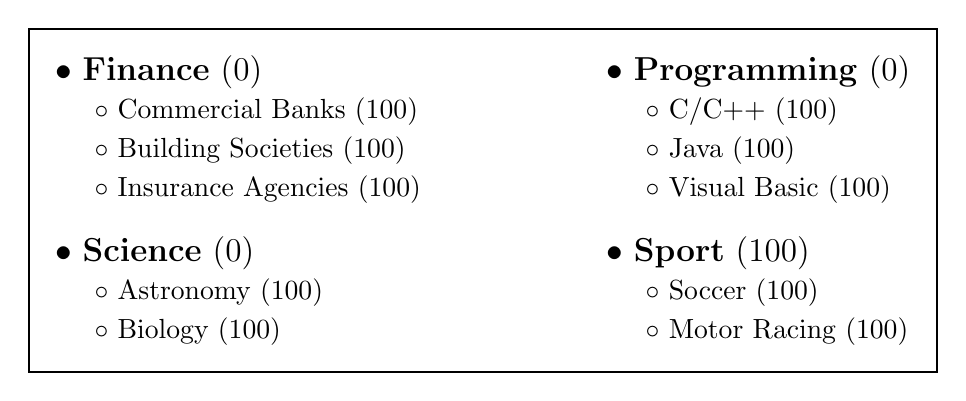
\begin{tikzpicture}[baseline=(current bounding box.north)]
  \usetikzlibrary{fit}

  % Left column
  \node (f1) [anchor=west] at (0.5,5.5) {\large$\bullet$ \textbf{Finance} (0)};
  \node (f2) [anchor=west] at (1.0,5.0) {$\circ$ Commercial Banks (100)};
  \node (f3) [anchor=west] at (1.0,4.5) {$\circ$ Building Societies (100)};
  \node (f4) [anchor=west] at (1.0,4.0) {$\circ$ Insurance Agencies (100)};

  \node (s1) [anchor=west] at (0.5,3.2) {\large$\bullet$ \textbf{Science} (0)};
  \node (s2) [anchor=west] at (1.0,2.7) {$\circ$ Astronomy (100)};
  \node (s3) [anchor=west] at (1.0,2.2) {$\circ$ Biology (100)};

  % Right column
  \node (p1) [anchor=west] at (7.5,5.5) {\large$\bullet$ \textbf{Programming} (0)};
  \node (p2) [anchor=west] at (8.0,5.0) {$\circ$ C/C++ (100)};
  \node (p3) [anchor=west] at (8.0,4.5) {$\circ$ Java (100)};
  \node (p4) [anchor=west] at (8.0,4.0) {$\circ$ Visual Basic (100)};

  \node (sp1) [anchor=west] at (7.5,3.2) {\large$\bullet$ \textbf{Sport} (100)};
  \node (sp2) [anchor=west] at (8.0,2.7) {$\circ$ Soccer (100)};
  \node (sp3) [anchor=west] at (8.0,2.2) {$\circ$ Motor Racing (100)};

  % Dynamic outer box (this replaces the fixed rectangle)
  \node[
    draw,
    line width=0.8pt,
    fit=(f1)(s3)(p1)(sp3),
    inner sep=6pt
  ] {};
\end{tikzpicture}%
}
\caption{Banksearch dataset \cite{bade_creating_2008}.}
\end{figure}






\subsection{Topic-Document Constraint Mapping}
\label{sec:topic_document_mapping}
In the BankSearch dataset, we do not have a hierarchical structure of documents, but rather on topics.
Hence, we extract \ac{mlb} constraints on the topic level, and map them to the document-level based on the topic assignments of the documents.
In this case, each document is associated with exactly one topic, allowing for a straightforward mapping of the generated \ac{mlb} constraints to document-level constraints. 
We chose to omit any \ac{mlb} constraints involving categories that do not have any assigned documents.
Instead of mapping each document to its assigned topic, we translate the topic-level \ac{mlb} constraints to document-level constraints of \textit{representative} documents and thus, reduce the number of constraints.
In other words: Each document belongs to an equivalence class defined by its assigned topic. 
We select one representative document from each topic to serve as a proxy for the entire class in the constraint mapping.
% We denote this \textit{clarified} context, but expand the resulting lattices with the remaining documents for later analysis.
For instance, if documents $d_x$, $d_y$, and $d_z$ are labeled with topics $x$, $y$, and $z$ respectively, then the MLB constraint $(x,y,z)$ directly translates to a document-level constraint $(d_x, d_y, d_z)$.
One the BankSearch dataset, this results in $81$ \ac{mlb} constraints, which are then used to construct the formal context for the \ac{mlb}-informed concept lattice.

% \input{chapters/08_case_study/dendogram_effectiveness_measure.tex}

\subsection{Comparison of Resulting Concept Lattices}
\label{sec:lattice_comparison}


The two lattices are constructed over the same object set of 11\,000 documents. 
The \ac{mlb}-constrained lattice in Figure~\ref{fig:mlb_concept_lattice} contains all concepts, the topic model-based lattice in Figure~\ref{fig:iceberg_concept_lattice} is computed as an iceberg lattice, retaining only concepts whose intents satisfy a minimum support threshold. 
This restriction is necessary because the complete topic model-based lattice contains more than 550 concepts (Figure~\ref{fig:concepts_support}), which would hinder visualization and interpretation.

\begin{figure}[t]
    \centering
    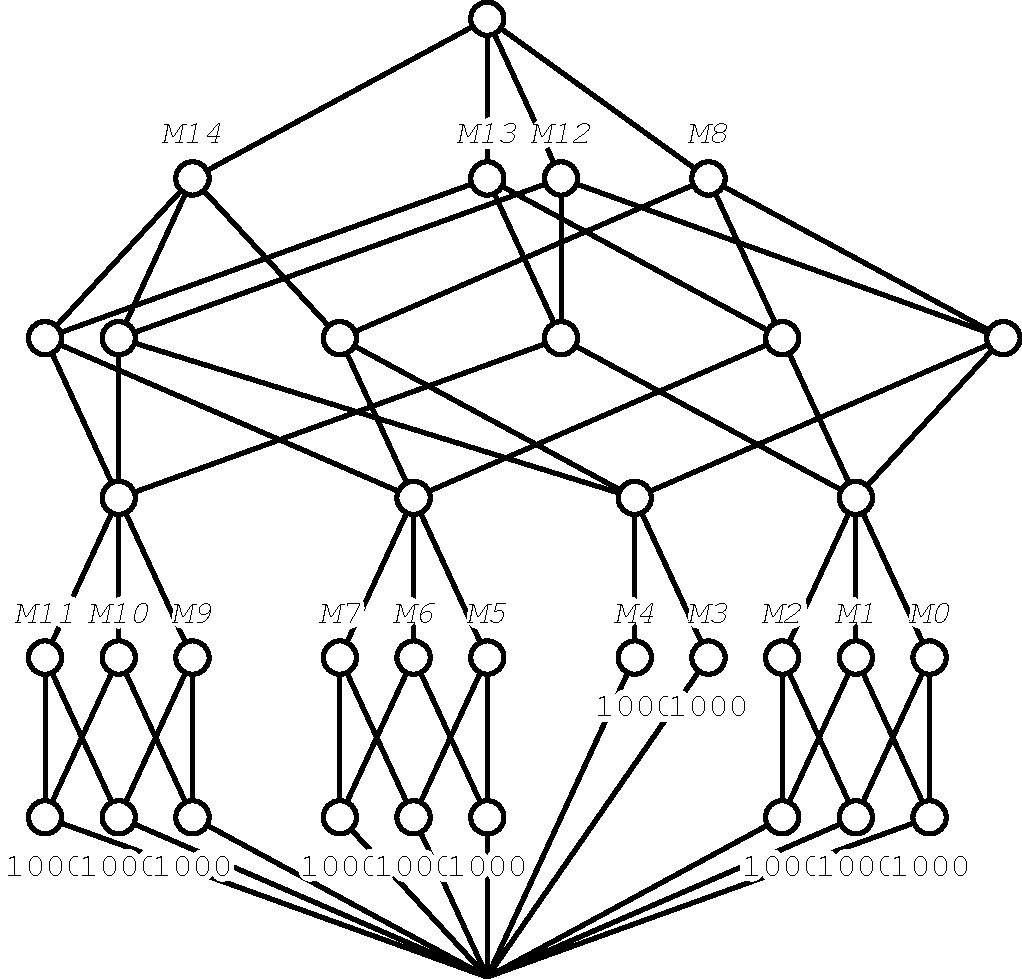
\includegraphics[width=0.6\textwidth]{resources/banksearch/ground_truth/mlb_expanded.pdf}
    \caption{\ac{mlb}-constrained concept lattice. Top labels denote attributes; bottom labels indicate the number of documents in the corresponding concept extent. Evaluation against manually annotated ground-truth labels indicates that numbered nodes correspond to document clusters sharing the same topic.} % kind of obvious, because that is the smallest attribute set they share
    \label{fig:mlb_concept_lattice}
\end{figure}

In the \ac{mlb}-constrained concept lattice (Figure~\ref{fig:mlb_concept_lattice}), attributes are labeled $M_i$ as generated by the script constructing the formal context from the \ac{mlb} constraints. 
The lattice contains 15 attributes, of which only $M3$ and $M4$ correspond directly to ground-truth topics (\texttt{Biology} and \texttt{Astronomy}). 
This correspondence was identified by matching concept extents to the original topic assignments.
Most remaining topics emerge as intersections of attributes; for example, \texttt{Sport} corresponds to $M0 \cap M1$, while \texttt{Soccer} and \texttt{Motor Racing} correspond to $M1 \cap M2$ and $M0 \cap M2$, respectively.
Consequently, most original topics appear near the bottom of the lattice.

\begin{figure}[t]
    \centering
    \includesvg[width=\textwidth]{resources/banksearch/topic_model/banksearch_0.05_iceberg.svg}
    \caption{Iceberg concept lattice derived from the topic model. Top labels denote cluster IDs in the concept intent; bottom labels indicate the number of documents in the concept extent.}
    \label{fig:iceberg_concept_lattice}
\end{figure}

The topic model-based lattice (Figure~\ref{fig:iceberg_concept_lattice}) contains 24 concepts with support of at least $\delta_{ms}=0.05$. 
Unlike the \ac{mlb}-constrained lattice, the original dataset topics are not explicitly represented as individual concepts.
The iceberg lattice contains only two non-trivial levels besides the top and bottom concepts, resulting in substantially less hierarchical depth than the \ac{mlb}-constrained lattice due to iceberg pruning. 
This reduction in structure is expected due to the pruning effect of the iceberg constraint.

\begin{figure}[hbt]
    \centering
    \includesvg[width=0.64\textwidth]{results/context_comparison/CONCEPT_SIM/heatmap_0.05.svg}
    \caption{Pairwise Jaccard similarities between concept extents of the \ac{mlb}-constrained lattice and the topic model-based iceberg lattice. Apart from the trivial similarity of the top concepts, most pairs exhibit near-zero similarity. \textcolor{red}{TODO: update path dep. on min-supp}}
    \label{fig:concept_lattice_similarity}
\end{figure}

% Glckstad2013UnsupervisedKS use Jaccard for overlapping intents
To compare both lattices, we compute the Jaccard similarity~\cite{Glckstad2013UnsupervisedKS} between all pairs of concept extents.
For extents $A$ and $B$, the similarity is defined as $J(A,B) = \frac{|A \cap B|}{|A \cup B|}$.
Figure~\ref{fig:concept_lattice_similarity} shows that most similarities are close to zero, indicating minimal overlap between document clusters.
Excluding the trivial similarity of the top concepts, only \textcolor{red}{three} concept pairs reach a similarity above $0.6$ (Table~\ref{tab:concept_jaccard_similarity}). 
These pairs correspond to concepts located in the middle region of the \ac{mlb}-constrained lattice. 
For example, the concept generated by $A'{M4, M8, M12, M14}$ (at the $m4$ node \texttt{Astronomy}), aligns most closely with topic-model concept $c10$, which captures computer science-related topic words.
Overall, the two lattices exhibit very limited structural similarity.

%% min-sup = 0.1
\begin{table}[b]
\centering
% Jaccard is defined on extent, therefore we compare J(A,B) but refer to the intents as concept identifiers
\caption{Concept pairs with Jaccard similarity above $0.6$, where $A'$ denotes the \ac{mlb}-constrained concept intent and $B'$ the topic model-based concept intent. \textcolor{red}{update with min-supp=0.05, ggf. new computation cf. Fig. 7?}}
\label{tab:concept_jaccard_similarity}
\begin{tabular}{lll}
\toprule
$A'$ & $B'$ & $J(A,B)$ \\
\midrule
$\{M12, M13, M14\}$ & $\{c7\}$ & 0.77 \\
$\{M1, M8, M12, M13\}$  & $\{c9\}$ & 0.65 \\
$\{M4, M8, M12, M14\}$  & $\{c10\}$ & 0.64 \\
\bottomrule
\end{tabular}
\end{table}



\subsection{Consistency-Lattice vs. Coherence-Lattice}
\label{sec:consistency_vs_coherence}

The consistency lattice in Figure~\ref{fig:consistency_coherence_lattices} (left) is computed by intersecting the \ac{mlb}-constrained lattice with the lattice derived from the topic model, following the procedure described in Section~\ref{sec:integrated_lattice_computation}.
Formally, $\mathcal{C}_{\cap} = \mathcal{C}_{\Sigma} \cap \mathcal{C}_{TM}$. In our case, this intersection is near-trivial, containing only the top and bottom concepts.
To investigate partial overlaps, we define the \textit{coherence-lattice} $\mathfrak{B}(\mathbb{K}_{coh})$. We construct a new formal context $\mathbb{K}_{coh} = (G, M_{coh}, I_{coh})$, where the attributes $M_{coh}$ are derived from pairs of concepts $(A, B)$ with $A \in \mathcal{C}_{\Sigma}$ and $B \in \mathcal{C}_{TM}$ that satisfy a Jaccard threshold $\theta$:
\begin{equation}
    M_{coh} = \{ A \cap B \mid A \in \mathcal{C}_{\Sigma}, B \in \mathcal{C}_{TM}, J(A, B) > \theta \}
\end{equation}
We set $\theta = 0.6$ which allows us to visualize document clusters that are \textit{nearly} consistent across both knowledge sources.
Since the top node of the coherence lattice contains $11\,000$ documents the resulting lattice covers the complete corpus.

\begin{figure}[t]
\centering

\begin{subfigure}{0.45\textwidth}
    \centering
    \includesvg[width=0.35\textwidth]{results/context_comparison/intersection.svg}
    % \caption{\textit{Consistency}-lattice.}
\end{subfigure}
\hfill
\begin{subfigure}{0.45\textwidth}
    \centering
    \includesvg[width=0.7\textwidth]{results/context_comparison/CONCEPT_SIM/coherence.svg}
    % \caption{\textit{Coherence}-lattice.}
\end{subfigure}

\caption{The \emph{consistency} lattice (left) and \emph{coherence} lattice (right) from the \ac{mlb}-constrained lattice and the topic model-based lattice for the BankSearch dataset.}
\label{fig:consistency_coherence_lattices}

\end{figure}


\section{Conclusion and Future Work}
\label{sec:future_work}

The analysis of the consistency- and coherence-lattices highlights the distinction between strict and relaxed notions of agreement between knowledge bases. 
The consistency-lattice retains only concepts whose extents coincide exactly in both the \ac{mlb}-constrained and the topic model-based lattices. 
In our experiments, no non-trivial document clusters were shared exactly between the two lattices. %, indicating that strict consistency is often too restrictive when comparing knowledge bases derived from heterogeneous sources.
% limitation
Generally, pruning low-support concepts through iceberg filtering can remove exact overlaps and thus yield an incomplete consistency-lattice. 
Thus, it is important to design the pipeline data-dependent to avoid this issue.
% However, in our experiments, the absence of non-trivial shared concepts appears to reflect genuine semantic differences between the expert-defined and topic model-based knowledge bases rather than an artefact of pruning.

The empty consistency-lattice refelcts fundamental differences between the two knowledge bases.
The \ac{mlb}-constrained lattice is derived from manual annotations and thus reflects human expertise, preferences and biases, while the topic model-based lattice is data-driven and captures latent statistical regularities and noise in the corpus, potentially revealing structures not explicitly encoded in the manual taxonomy.
Our approach allows for the integration of alternative topic modeling methods.

Our study provides two main contributions. 
First, we showed that \ac{mlb} constraints can be integrated natively into the \ac{fca} framework through a fixpoint-based closure operator. 
Second, experiments on the BankSearch dataset demonstrated that exact consistency between manual hierarchies and data-driven topic models is rarely observed in real-world corpora.

In practice, this implies that a multi-tier approach is necessary: (1) using the \textit{consistency-lattice} to identify undisputed common ground and (2) utilizing the \textit{coherence-lattice} with tunable thresholds to explore meaningful alignments. 

The coherence-lattice addresses this limitation by building document clusters based on partial overlaps between concept extents through a similarity threshold.  
Moreover, the number of documents contained in coherence-lattice concepts provides an indication of the degree of agreement between the underlying representations.

Overall, the results suggest that practical knowledge integration requires tolerating a certain degree of inconsistency while maintaining sufficient coherence. 
The appropriate similarity threshold depends on the application domain: safety-critical settings such as medicine may require high thresholds to ensure reliable alignment, whereas exploratory analysis may benefit from lower thresholds that permit broader, though less precise, overlaps.

Future work will investigate the integration of more than two knowledge bases, methods for selecting similarity thresholds that yield coherence-lattices of comparable size, and alternative overlap measures beyond Jaccard similarity for comparing concept extents across multiple lattices.

% ---- Acronyms ----
\begin{acronym}
    \acro{fca}[FCA]{Formal Concept Analysis}
    \acro{nlp}[NLP]{Natural Language Processing}
    \acro{hdbscan}[HDBSCAN]{Hierarchical Density-Based Spatial Clustering of Applications with Noise}
    \acro{bow}[BoW]{Bag of Words}
    \acro{tfidf}[TF-IDF]{Term Frequency-Inverse Document Frequency}
\end{acronym}


% ---- Bibliography ----

% BibTeX users should specify bibliography style 'splncs04'.
% References will then be sorted and formatted in the correct style.
\bibliographystyle{splncs04}
\bibliography{bibliography}

\newpage
\input{chapters/10_appendix}

\end{document}
